@ -1,1111 +0,0 @@
% *** Authors should verify (and, if needed, correct) their LaTeX system  ***
% *** with the testflow diagnostic prior to trusting their LaTeX platform ***
% *** with production work. IEEE's font choices can trigger bugs that do  ***
% *** not appear when using other class files.                            ***
% The testflow support page is at:
% http://www.michaelshell.org/tex/testflow/


%%*************************************************************************
%% Legal Notice:
%% This code is offered as-is without any warranty either expressed or
%% implied; without even the implied warranty of MERCHANTABILITY or
%% FITNESS FOR A PARTICULAR PURPOSE!
%% User assumes all risk.
%% In no event shall IEEE or any contributor to this code be liable for
%% any damages or losses, including, but not limited to, incidental,
%% consequential, or any other damages, resulting from the use or misuse
%% of any information contained here.
%%
%% All comments are the opinions of their respective authors and are not
%% necessarily endorsed by the IEEE.
%%
%% This work is distributed under the LaTeX Project Public License (LPPL)
%% ( http://www.latex-project.org/ ) version 1.3, and may be freely used,
%% distributed and modified. A copy of the LPPL, version 1.3, is included
%% in the base LaTeX documentation of all distributions of LaTeX released
%% 2003/12/01 or later.
%% Retain all contribution notices and credits.
%% ** Modified files should be clearly indicated as such, including  **
%% ** renaming them and changing author support contact information. **
%%
%% File list of work: IEEEtran.cls, New_IEEEtran_how-to.pdf, bare_jrnl_new_sample4.tex,
%%*************************************************************************
\PassOptionsToPackage{unicode}{hyperref}
\PassOptionsToPackage{hyphens}{url}
\PassOptionsToPackage{dvipsnames,svgnames,x11names}{xcolor}
% Note that the a4paper option is mainly intended so that authors in
% countries using A4 can easily print to A4 and see how their papers will
% look in print - the typesetting of the document will not typically be
% affected with changes in paper size (but the bottom and side margins will).
% Use the testflow package mentioned above to verify correct handling of
% both paper sizes by the user's LaTeX system.
%
% Also note that the "draftcls" or "draftclsnofoot", not "draft", option
% should be used if it is desired that the figures are to be displayed in
% draft mode.
%
\documentclass[
  lettersize  journal,
]{IEEEtran}%
% If IEEEtran.cls has not been installed into the LaTeX system files,
% manually specify the path to it like:
% \documentclass[journal]{../sty/IEEEtran}
%\usepackage[cmex10]{amsmath}
%\usepackage{amssymb}
\usepackage{iftex}
\usepackage{subcaption}
\renewcommand{\thesubfigure}{(\alph{subfigure})}
\captionsetup[subfigure]{labelformat=simple}
\usepackage{caption}
\captionsetup[table]{justification=centerlast, labelsep=newline, textfont={small,sc}}
\ifPDFTeX
  \usepackage[T1]{fontenc}
  \usepackage[utf8]{inputenc}
  \usepackage{textcomp} % provide euro and other symbols
\else % if luatex or xetex
  \usepackage{unicode-math} % this also loads fontspec
  \defaultfontfeatures{Scale=MatchLowercase}
  \defaultfontfeatures[\rmfamily]{Ligatures=TeX,Scale=1}
\fi
%\usepackage{lmodern}
\ifPDFTeX\else
\fi
% Use upquote if available, for straight quotes in verbatim environments
\IfFileExists{upquote.sty}{\usepackage{upquote}}{}
\IfFileExists{microtype.sty}{% use microtype if available
  \usepackage[]{microtype}
  \UseMicrotypeSet[protrusion]{basicmath} % disable protrusion for tt fonts
}{}
\makeatletter
\parindent    1.0em
\ifCLASSOPTIONcompsoc
  \parindent    1.5em
\fi
\makeatother
\usepackage{xcolor}
\setlength{\emergencystretch}{3em} % prevent overfull lines

\setcounter{secnumdepth}{5}
% Make \paragraph and \subparagraph free-standing
\ifx\paragraph\undefined\else
  \let\oldparagraph\paragraph
  \renewcommand{\paragraph}[1]{\oldparagraph{#1}\mbox{}}
\fi
\ifx\subparagraph\undefined\else
  \let\oldsubparagraph\subparagraph
  \renewcommand{\subparagraph}[1]{\oldsubparagraph{#1}\mbox{}}
\fi


\providecommand{\tightlist}{%
  \setlength{\itemsep}{0pt}\setlength{\parskip}{0pt}}\usepackage{longtable,booktabs,array}
\usepackage{calc} % for calculating minipage widths
% Correct order of tables after \paragraph or \subparagraph
\usepackage{etoolbox}
\makeatletter
\patchcmd\longtable{\par}{\if@noskipsec\mbox{}\fi\par}{}{}
\makeatother
% Allow footnotes in longtable head/foot
\IfFileExists{footnotehyper.sty}{\usepackage{footnotehyper}}{\usepackage{footnote}}
\makesavenoteenv{longtable}
\usepackage{graphicx}
\makeatletter
\def\maxwidth{\ifdim\Gin@nat@width>\linewidth\linewidth\else\Gin@nat@width\fi}
\def\maxheight{\ifdim\Gin@nat@height>\textheight\textheight\else\Gin@nat@height\fi}
\makeatother
% Scale images if necessary, so that they will not overflow the page
% margins by default, and it is still possible to overwrite the defaults
% using explicit options in \includegraphics[width, height, ...]{}
\setkeys{Gin}{width=\maxwidth,height=\maxheight,keepaspectratio}
% Set default figure placement to htbp
\makeatletter
\def\fps@figure{htbp}
\makeatother
% definitions for citeproc citations
\NewDocumentCommand\citeproctext{}{}
\NewDocumentCommand\citeproc{mm}{%
  \begingroup\def\citeproctext{#2}\cite{#1}\endgroup}
\makeatletter
 % allow citations to break across lines
 \let\@cite@ofmt\@firstofone
 % avoid brackets around text for \cite:
 \def\@biblabel#1{}
 \def\@cite#1#2{{#1\if@tempswa , #2\fi}}
\makeatother
\newlength{\cslhangindent}
\setlength{\cslhangindent}{1.5em}
\newlength{\csllabelwidth}
\setlength{\csllabelwidth}{3em}
\newenvironment{CSLReferences}[2] % #1 hanging-indent, #2 entry-spacing
 {\begin{list}{}{%
  \setlength{\itemindent}{0pt}
  \setlength{\leftmargin}{0pt}
  \setlength{\parsep}{0pt}
  % turn on hanging indent if param 1 is 1
  \ifodd #1
   \setlength{\leftmargin}{\cslhangindent}
   \setlength{\itemindent}{-1\cslhangindent}
  \fi
  % set entry spacing
  \setlength{\itemsep}{#2\baselineskip}}}
 {\end{list}}
\usepackage{calc}
\newcommand{\CSLBlock}[1]{\hfill\break\parbox[t]{\linewidth}{\strut\ignorespaces#1\strut}}
\newcommand{\CSLLeftMargin}[1]{\parbox[t]{\csllabelwidth}{\strut#1\strut}}
\newcommand{\CSLRightInline}[1]{\parbox[t]{\linewidth - \csllabelwidth}{\strut#1\strut}}
\newcommand{\CSLIndent}[1]{\hspace{\cslhangindent}#1}

\usepackage{booktabs}
\usepackage{longtable}
\usepackage{array}
\usepackage{multirow}
\usepackage{wrapfig}
\usepackage{float}
\usepackage{colortbl}
\usepackage{pdflscape}
\usepackage{tabu}
\usepackage{threeparttable}
\usepackage{threeparttablex}
\usepackage[normalem]{ulem}
\usepackage{makecell}
\usepackage{xcolor}
\usepackage{physics}
\usepackage[version=3]{mhchem}
\usepackage{orcidlink}
\usepackage{float} 
\usepackage{bm,bbm}
\usepackage{mathrsfs}
\usepackage{nccmath}
\usepackage{amssymb}
\usepackage{mathtools}
\usepackage{siunitx}
\usepackage{graphicx}
\usepackage{url}
\usepackage[T1]{fontenc}
\usepackage{booktabs}
\usepackage{color}
\usepackage{hyperref}
\usepackage{float}
\usepackage{array}
\usepackage{multirow}
\usepackage{wrapfig}
\usepackage{colortbl}
\usepackage{pdflscape}
\usepackage{xcolor}
\makeatletter
\@ifpackageloaded{caption}{}{\usepackage{caption}}
\AtBeginDocument{%
\ifdefined\contentsname
  \renewcommand*\contentsname{Table of contents}
\else
  \newcommand\contentsname{Table of contents}
\fi
\ifdefined\listfigurename
  \renewcommand*\listfigurename{List of Figures}
\else
  \newcommand\listfigurename{List of Figures}
\fi
\ifdefined\listtablename
  \renewcommand*\listtablename{List of Tables}
\else
  \newcommand\listtablename{List of Tables}
\fi
\ifdefined\figurename
  \renewcommand*\figurename{Fig.}
\else
  \newcommand\figurename{Fig.}
\fi
\ifdefined\tablename
  \renewcommand*\tablename{Table}
\else
  \newcommand\tablename{Table}
\fi
}
\@ifpackageloaded{float}{}{\usepackage{float}}
\floatstyle{ruled}
\@ifundefined{c@chapter}{\newfloat{codelisting}{h}{lop}}{\newfloat{codelisting}{h}{lop}[chapter]}
\floatname{codelisting}{Listing}
\newcommand*\listoflistings{\listof{codelisting}{List of Listings}}
\makeatother
\makeatletter
\makeatother
\makeatletter
\@ifpackageloaded{caption}{}{\usepackage{caption}}
\@ifpackageloaded{subcaption}{}{\usepackage{subcaption}}
\makeatother
\usepackage[skip=2pt,font=footnotesize]{caption}
%\captionsetup{format=myformat}
\makeatletter
%\setlength{\cslhangindent}{0pt plus .5pt}
\providecommand{\bibfont}{\footnotesize}
\let\CSLReferences@rig=\CSLReferences
\renewcommand{\CSLReferences}[2]{
\bibfont\settowidth\csllabelwidth{[999]}
\CSLReferences@rig{#1}{#2}
\vskip 0.3\baselineskip plus 0.1\baselineskip minus 0.1\baselineskip%
}
\makeatother
\ifLuaTeX
  \usepackage{selnolig}  % disable illegal ligatures
\fi
\IfFileExists{bookmark.sty}{\usepackage{bookmark}}{\usepackage{hyperref}}
\IfFileExists{xurl.sty}{\usepackage{xurl}}{} % add URL line breaks if available
\urlstyle{same} % disable monospaced font for URLs
\hypersetup{
  pdftitle={Quantifying Heterogeneity in SAR Imagery with the Rényi Entropy},
  pdfauthor={Janeth Alpala; Abraão D.~C.~Nascimento; Alejandro C.~Frery},
  pdfkeywords={Rényi entropy, Gamma
distribution, heterogeneity, SAR, hypothesis tests, bootstrap},
  colorlinks=true,
  linkcolor={black},
  filecolor={Maroon},
  citecolor={black},
  urlcolor={black},
  pdfcreator={LaTeX via pandoc}}

% *** Do not adjust lengths that control margins, column widths, etc. ***
% *** Do not use packages that alter fonts (such as pslatex).         ***
% There should be no need to do such things with IEEEtran.cls V1.6 and later.
% (Unless specifically asked to do so by the journal or conference you plan
% to submit to, of course. )


% correct bad hyphenation here
\hyphenation{op-tical net-works semi-conduc-tor}

%
% paper title
% can use linebreaks \\ within to get better formatting as desired
% Do not put math or special symbols in the title.
% paper title
% can use linebreaks \\ within to get better formatting as desired
% Do not put math or special symbols in the title.
\title{Quantifying Heterogeneity in SAR Imagery with the Rényi Entropy}

\author{
Janeth Alpala\orcidlink{0000-0002-0265-6236},~Abraão
D.~C.~Nascimento\orcidlink{0000-0003-2673-219X}
and~Alejandro
C.~Frery\orcidlink{0000-0002-8002-5341},~\IEEEmembership{Fellow, IEEE}%
\thanks{Janeth Alpala and Abraão D. C. Nascimento are with the
Departamento de Estatística, Universidade Federal de Pernambuco, Recife,
50670-901 PE, Brazil (e-mails: janeth.alpala@ufpe.br,
abraao@de.ufpe.br).

Alejandro C. Frery is with the School of Mathematics and Statistics,
Victoria University of Wellington, Wellington, 6140, New Zealand
(e-mail: alejandro.frery@vuw.ac.nz).
\emph{Corresponding author: Alejandro C. Frery.}

Data and code are available at:
\url{https://github.com/rjaneth/renyi-entropy}}
}
\begin{document}

% The paper headers
\markboth{Journal XXX, Month Year}{}

% use for special paper notices

% make the title area
\maketitle

% As a general rule, do not put math, special symbols or citations
% in the abstract or keywords.
\begin{abstract}
Quantifying surface roughness in synthetic aperture radar (SAR) data is
critical for accurate geophysical interpretation and remote sensing
applications. We propose a test statistic based on a non-parametric
estimation of Rényi entropy to characterize surface roughness from SAR
intensity data. The statistic is refined using bootstrap to improve its
stability, size, and power. This approach enhances roughness
quantification by capturing scale-dependent variations and addressing
data-driven uncertainty. Experimental results demonstrate the robustness
of the proposed method in distinguishing roughness patterns.
\end{abstract}
% Note that keywords are not normally used for peerreview papers.
\begin{IEEEkeywords}
Rényi entropy, Gamma distribution, heterogeneity, SAR, hypothesis
tests, bootstrap
\end{IEEEkeywords}

% For peer review papers, you can put extra information on the cover
% page as needed:
% \ifCLASSOPTIONpeerreview
% \begin{center} \bfseries EDICS Category: 3-BBND \end{center}
% \fi
%
% For peerreview papers, this IEEEtran command inserts a page break and
% creates the second title. It will be ignored for other modes.
% \IEEEpeerreviewmaketitle


\renewcommand{\tablename}{TABLE}

\section{Introduction}\label{introduction}

\IEEEPARstart{S}{ynthetic} Aperture Radar (SAR) technology has become
essential for many applications~\citeproc{ref-Mondini2021}{{[}1{]}}. It
provides high-resolution data independent of sunlight and operates in
various weather conditions, facilitating global Earth
monitoring~\citeproc{ref-Zeng2020}{{[}2{]}}. However, the effective use
of SAR data depends on understanding its statistical properties because
it is affected by speckle, a noise-like interference
effect~\citeproc{ref-Baraha2023}{{[}3{]}}. In intensity format, speckle
is non-Gaussian, which complicates image analysis.

The \(\mathcal{G}^0_I\) distribution effectively characterizes SAR
intensity data because it captures different roughness levels. A
limiting case is the Gamma distribution, associated with fully developed
speckle in textureless regions. However, selecting suitable models is
challenging due to small window sizes in practical applications and
difficulties in parameter estimation, motivating alternative statistical
approaches.

Entropy measures have gained attention for SAR analysis, with
applications in edge detection~\citeproc{ref-Nascimento2014}{{[}4{]}},
segmentation~\citeproc{ref-Nobre2016}{{[}5{]}}, and noise
reduction~\citeproc{ref-Chan2022}{{[}6{]}}. Traditionally, Shannon
entropy~\citeproc{ref-Shannon1948}{{[}7{]}} has been widely used to
quantify data uncertainty and disorder. We explore a more general
information measure: Rényi entropy---a generalization of Shannon's
formulation.

\textcolor{blue}{Recent studies highlight the role of entropy in SAR classification.
Cassetti et al.~\citeproc{ref-Cassetti2022}{{[}8{]}} evaluated entropy
estimators in both supervised and unsupervised models. Gallet et al.~\citeproc{ref-Gallet2024}{{[}9{]}} 
proposed a Rényi divergence-based
framework for explainable classification. Parikh et al.~\citeproc{ref-Parikh2019}{{[}10{]}} discussed challenges in deep
learning for SAR, including limited availability of labeled data and the
complexity of tuning hyperparameters. These works motivate lightweight,
interpretable alternatives.}

We propose a statistical test based on a non-parametric estimator of
Rényi entropy to identify heterogeneous regions in SAR data. The test
assesses whether the observed Rényi entropy significantly differs from
its expected theoretical value under the homogeneity assumption,
improving upon our previous Shannon-based
approach~\citeproc{ref-Frery2024}{{[}11{]}}.
\textcolor{blue}{We further enhance the non-parametric estimator through a bootstrap-based bias correction, improving accuracy for small windows.}
\textcolor{blue}{The proposed approach is unsupervised, requires no training data, and yields interpretable $p$-values, making it especially suitable for scenarios where ground truth information is limited or unavailable.}

The rest of this article is organized as follows. Section~\ref{sec:pre}
overviews the statistical models for SAR intensity data and Rényi
entropy. Section~\ref{sec:met} describes the proposed hypothesis test.
Section~\ref{sec:app} evaluates the performance of the test using SAR
data. Finally, the conclusions are presented in
Section~\ref{sec:conclusion}.

\section{PRELIMINARIES}\label{sec:pre}

\subsection{Statistical Models}\label{statistical-models}

The main distributions considered for SAR intensity data are the
\(\Gamma_{\text{SAR}}\) distribution, which is suitable for fully
developed speckle, and the \(\mathcal{G}^0_I\) distribution, which can
describe roughness~\citeproc{ref-Frery1997}{{[}12{]}}. These
distributions are characterized by the following probability density
functions (pdfs): \begin{equation}
    f_{\Gamma_{\text{SAR}}}\bigl(z;L, \mu \bigr) 
    = \frac{L^L}{\Gamma(L)\,\mu^L} z^{L-1} 
    \exp \biggl(-\frac{Lz}{\mu}\biggr)
    \mathbbm 1_{\mathbbm R_+}(z) \label{E:gamma1}
\end{equation} and \begin{multline}
    f_{\mathcal{G}^0_I}\bigl(z; \mu, \alpha, L \bigr) 
    = \frac{L^L\,\Gamma(L-\alpha)}
    {\bigl[-\mu(\alpha+1)\bigr]^{\alpha} \Gamma(-\alpha)\,\Gamma(L)}\\
    \frac{z^{L-1}}
    {\bigl[-\mu(\alpha+1)+Lz\bigr]^{L-\alpha}}
    \mathbbm 1_{\mathbbm R_+}(z), \label{E:gi01}
\end{multline} where \(\mu > 0\) is the mean, \(\alpha < 0\) measures
the roughness, \(L \geq 1\) is the number of looks, \(\Gamma(\cdot)\) is
the gamma function, and \(\mathbbm 1_{A}(z)\) is the indicator function
of the set \(A\). The \(\Gamma_{\text{SAR}}\) law is a particular case
of the \(\mathcal{G}^0_I\)
distribution~\citeproc{ref-Frery1997}{{[}12{]}}: for \(\mu\) fixed, \[
f_{\mathcal{G}^0_I}\big(z; \mu, \alpha, L\big)
\longrightarrow 
f_{\Gamma_{\text{SAR}}}(z;L, \mu) \text{ when } \alpha\to-\infty.
\]

\subsection{Rényi Entropy}\label{ruxe9nyi-entropy}

For a continuous random variable \(Z\) with pdf \(f(z)\), the Rényi
entropy of order \(\lambda \in \mathbbm R_+ \setminus \{1\}\) is defined
as: \begin{equation}
\label{E:entropy2}
H_\lambda(Z) = \frac{1}{1 - \lambda} \ln \int_{-\infty}^{\infty} [f(z)]^\lambda \, dz.
\end{equation} Using~\eqref{E:entropy2}, we derive closed-form
expressions for the Rényi entropy of the \(\Gamma_{\mathrm{SAR}}\) and
the \(\mathcal{G}^0_I\) distributions: \begin{multline}
\label{eq-HGammaSAR}
H_\lambda\bigl(\Gamma_{\text{SAR}}(L, \mu)\bigr)
= 
\ln \mu - \ln L + \frac{1}{1-\lambda}
\Bigl[
  -\lambda\,\ln\Gamma(L)  \\ + \ln\Gamma\bigl(\lambda(L-1)+1\bigr)  - \bigl(\lambda(L-1)+1\bigr)\,\ln\lambda
\Bigr]
\end{multline} and \begin{multline}  
\label{eq-HGI0}  
H_\lambda\bigl(\mathcal{G}^0_I(\mu, \alpha, L)\bigr) = H_\lambda\bigl(\Gamma_{\text{SAR}}(L, \mu)\bigr) \;\;+ \\ \ln(-1 - \alpha)  
+ \frac{1}{1 - \lambda} \Bigl[ \lambda\bigl(\ln\Gamma(L - \alpha) - \ln\Gamma(-\alpha)\bigr) \\ 
+ \ln\Gamma\bigl(\lambda(-\alpha + 1) - 1\bigr) - \ln\Gamma\bigl(\lambda(L - \alpha)\bigr) \\
+ \bigl(\lambda(L-1)+1\bigr)\ln\lambda \Bigr].  
\end{multline}
\textcolor{blue}{ Equation~\eqref{eq-HGI0} can be read as: 
\[
H_{\lambda}(\mathcal{G}^0_I)
=
\underbrace{H_\lambda\!\bigl(\Gamma_{\mathrm{SAR}}\bigr)}_{\text{baseline entropy}}
\hspace{1.8em} + \hspace{-1.0em}
\underbrace{\Delta_\alpha}_{\text{extra entropy caused by texture}}\hspace{-3.0em},
\]}

\textcolor{blue}{where the excess term $\Delta_\alpha$ depends on the roughness parameter.
When $\alpha\!\to\!-\infty$ (fully developed speckle), this excess tends to zero,
%<!-- , so the heterogeneous model collapses to the homogeneous one in Equation \eqref{eq-HGammaSAR}.  -->
and detecting heterogeneity is equivalent to deciding whether $\Delta_\alpha$ is significantly different from zero.
Fig.~\ref{fig-convergence} illustrates this behaviour: as \(\alpha\)
decreases the colored curves of \(H_\lambda(\mathcal{G}^0_I)\) converge
towards the solid black curve of \(H_\lambda(\Gamma_{\mathrm{SAR}})\).}

\begin{figure}[hbt]
  \centering
  \includegraphics[width=0.42\textwidth]{Figures-R1/fig-convergence-1.pdf}
  \vspace{0.5em}
  \caption{Convergence of $H_{\lambda}(\mathcal{G}^0_I)$ to $H_{\lambda}(\Gamma_{\text{SAR}})$ as $\alpha$ decreases.}
  \label{fig-convergence}
\end{figure}

\subsection{Non-parametric Estimation of Rényi
Entropy}\label{non-parametric-estimation-of-ruxe9nyi-entropy}

In order to estimate~\eqref{E:entropy2} from a random sample, one may
estimate the parameters that index the probability density function
\(f\) and integrate, an approach that relies on the model assumptions.
Recently, Al-Labadi et al.~\citeproc{ref-AlLabadi2024}{{[}13{]}}
proposed a non-parametric estimator for Rényi entropy based on
non-parametric estimation using differences between order statistics
(spacings).

Let \(\bm{Z}=(Z_1, Z_2,\ldots,Z_n)\) be an independent and identically
distributed random sample of size \(n\) from \(Z \sim F\), and let
\(Z_{(1)} \leq Z_{(2)} \leq \dots \leq Z_{(n)}\) denote its order
statistics. The \(m\)-spacing density estimator is defined as: \[
f_n(Z_{(i)}) = \frac{c_i m / n}{Z_{(i+m)} - Z_{(i-m)}},
\] where \(Z_{(i-m)} = Z_{(1)}\) when \(i \leq m\), and
\(Z_{(i+m)} = Z_{(n)}\) if \(i \geq n - m\). The coefficient \(c_i\) is
given by: \[
c_i = 
\begin{cases}
\frac{m + i - 1}{m}, & \text{if } 1 \leq i \leq m, \\%[6pt]
2, & \text{if } m+1 \leq i \leq n - m, \\%[6pt]
\frac{n + m - i}{m}, & \text{if } n - m + 1 \leq i \leq n.
\end{cases}
\] The Rényi entropy can be estimated with this density estimator as
\begin{align}
\label{eq:est_R}
\widehat{H}_\lambda(\bm{Z}) = \frac{1}{1 - \lambda} \ln \left[\frac{1}{n} \sum_{i=1}^{n} \left( \frac{c_i m / n}{Z_{(i+m)} - Z_{(i-m)}} \right)^{\lambda - 1} \right].
\end{align} This estimator is asymptotically consistent, i.e., it
converges in probability to the true value when \(m,n\rightarrow\infty\)
and \(m/n\rightarrow0\). We use the heuristic spacing
\(m=\left[\sqrt{n}+0.5\right]\).

\section{PROPOSED METHODOLOGY}\label{sec:met}

\subsection{\texorpdfstring{Finding an optimal value of
\(\lambda\)}{Finding an optimal value of \textbackslash lambda}}\label{finding-an-optimal-value-of-lambda}

\textcolor{blue}{
We aim to determine the optimal order $\lambda$ for the Rényi entropy estimator using simulated samples of size $n = 49$ from  $Z\sim \Gamma_{\text{SAR}}(5,1)$.
We computed the bias and the mean squared error (MSE) for varying $\lambda$ via a Monte Carlo experiment.
We found that for $L > 1$, $\lambda = 0.9$  yields the lowest MSE while maintaining a low bias, thus offering a favorable trade-off between bias and variance. 
As shown in Fig.~\ref{fig-optimal_order}, $\lambda = 0.85$ produces slightly lower bias, but results in higher MSE, supporting the choice of $\lambda = 0.9$.}

\begin{figure}[hbt]
  \centering
  \includegraphics[width=0.42\textwidth]{Figures-R1/fig-optimal_order-1.pdf}
  \vspace{0.5em}
  \caption{Bias and MSE as a function of $\lambda$, with $n=49$, $L=5$.}
  \label{fig-optimal_order}
\end{figure}

Particularly, for \(L = 1\), the optimal \(\lambda\) tends to be higher,
and we choose \(\lambda = 3\) to achieve good results.

\subsection{Bootstrap Correction for Entropy
Estimator}\label{bootstrap-correction-for-entropy-estimator}

Following Refs.~\citeproc{ref-Frery2024}{{[}11{]}},
\citeproc{ref-Alpala2024}{{[}14{]}}, we refine the non-parametric
entropy estimator \(\widehat{H}_{\lambda}\) in~\eqref{eq:est_R} with
bootstrap, obtaining \(\widetilde{H}_{\lambda}\): \begin{equation*}
\widetilde{H}_{\lambda} = 2\widehat{H}_{\lambda}(\bm{Z}) - \frac{1}{B} \sum_{b=1}^{B} \widehat{H}_{\lambda}(\bm{Z}^{(b)}),
\end{equation*} where \(B\) is the number of bootstrap replications, and
\(\bm{Z}^{(b)}\) denotes the \(b\)-th resampled dataset obtained by
drawing \(n\) observations with replacement from \(\bm{Z}\).

A Monte Carlo study with \(1000\) replications for each sample size
\(n \in \{9, 25, 49, 81, 121\}\) from the \(\Gamma_{\text{SAR}}\) (5,1)
confirms that for \(\lambda=0.9\), the bootstrap-corrected estimator
\(\widetilde{H}_{\lambda}\) (\(B=200\)) reduces both bias and MSE
compared to the original \(\widehat{H}_{\lambda}\), with significant
improvements for small sample sizes, as shown in Fig.~\ref{fig-bias_mse}.

\begin{figure}[hbt]
  \centering
  \includegraphics[width=0.40\textwidth]{Figures-R1/fig-bias_mse-1.pdf}
  \vspace{0.1em}
  \caption{Bias and MSE of the Rényi entropy estimators for $\Gamma_{\text{SAR}}$.}
  \label{fig-bias_mse}
\end{figure}

\subsection{Hypothesis Testing}\label{hypothesis-testing}

We test whether the observed data come from a homogeneous
(\(\Gamma_{\text{SAR}}\)) or a heterogeneous (\(\mathcal{G}^0_I\))
region, as follows: \begin{equation}\label{eq:hypothesis_test}
\begin{cases}
\mathcal{H}_0: \mathbb{E}[\widetilde{H}_{\lambda}] = H_{\lambda}(\Gamma_{\text{SAR}}) & \text{(Homogeneous region)}, \\[6pt]
\mathcal{H}_1: \mathbb{E}[\widetilde{H}_{\lambda}] = H_{\lambda}(\mathcal{G}^0_I) & \text{(Heterogeneous region)}.
\end{cases}
\end{equation}

Under \(\mathcal{H}_0\), the expected value of the entropy estimator
should match the theoretical \(H_{\lambda}(\Gamma_{\text{SAR}})\).
Significant deviations indicate heterogeneity.

\subsection{The Proposed Test}\label{the-proposed-test}

The test statistic quantifies the discrepancy between estimated and
theoretical entropy under homogeneity. Since \(L\geq1\) is known, we
define the test statistic as follows: \begin{multline}
\label{eq-test}
S_{\widetilde{H}_{\lambda}}(\bm{Z}; L) = \widetilde{H}_{\lambda} - \bigl\{\ln \widehat{\mu} - \ln L + \frac{1}{1-\lambda}
\bigl[-\lambda\,\ln\Gamma(L) \\ 
+ \ln\Gamma\bigl(\lambda(L-1)+1\bigr)  
- \bigl(\lambda(L-1)+1\bigr)\,\ln\lambda
\bigr]\bigr\},
\end{multline} where \(\widehat{\mu}={n}^{-1}\sum_{i=1}^n Z_{i}\) is the
sample mean.
\textcolor{blue}{The test statistic can be interpreted as: \[
S_{\widetilde H_\lambda} 
= 
\underbrace{\widetilde H_\lambda}_{\text{estimated}} 
\;-\;
\underbrace{H_\lambda\bigl(\Gamma_{\mathrm{SAR}}\bigr)}_{\text{theoretical under } H_0}\hspace{-0.5em},
\]
the difference between the estimated entropy and the expected value under homogeneity. Values close to zero indicate that the region behaves like fully developed speckle, while large positive values signal excess entropy and, thus, heterogeneity.
This formulation avoids the need to estimate $\mathcal{G}^0_I$ parameters  such as $\alpha$, offering a simple, interpretable, and statistically grounded test. Moreover, the method remains effective for small samples, aided by the bootstrap bias correction.}

Fig.~\ref{fig-densities} shows the empirical distribution of
\(S_{\widetilde{H}_{\lambda}}\) under \(\mathcal{H}_0\), obtained from
\(10^4\) Monte Carlo experiments with varying sample sizes
(\(n \in {49,81,121}\)), \(\lambda=0.9\), and \(L \in {5,18}\). 
\textcolor{blue}{The concentration around zero confirms the expected behavior of the test,
while the heavy tails indicate sensitivity to deviations, enabling the
detection of subtle texture changes.}

\begin{figure}[hbt]
  \centering
  \includegraphics[width=0.42\textwidth]{Figures-R1/fig-densities-1.pdf}
  \vspace{0.2em}
  \caption{Empirical densities of $S_{\widetilde{H}_{\lambda}}(\bm{Z}; L)$ under $\mathcal{H}_0$.}
  \label{fig-densities}
\end{figure}

Vasicek~\citeproc{ref-vasicek1976test}{{[}15{]}} proved that, for
sufficiently large samples, \(S_{\widetilde{H}_{\lambda}}(\bm{Z}; L)\)
asymptotically follows a normal distribution: \begin{equation*}
S_{\widetilde{H}_{\lambda}}(\bm{Z}; L) 
\overset{\mathcal{D}}{\underset{n \to \infty}{\longrightarrow}} 
\mathcal{N}(\mu_S,\,\sigma^{2}_S),
\end{equation*} where \(\mathcal{D}\) represents convergence in
distribution. Here,
\(\mu_S  = \mathbb{E}[S_{\widetilde{H}_{\lambda}}(\bm{Z}; L)]\) and
\(\sigma^{2}_S = \text{Var}[S_{\widetilde{H}_{\lambda}}(\bm{Z}; L)]\)
are the theoretical mean and variance of
\(S_{\widetilde{H}_{\lambda}}(\bm{Z}; L)\).

The standardized test statistic
\(\varepsilon = ({S_{\widetilde{H}_{\lambda}}(\bm{Z}; L) - \widehat{\mu}_S})/{\widehat{\sigma}_S}\)
is asymptotically standard normal distributed, where \(\widehat{\mu}_S\)
and \(\widehat{\sigma}_S\) are the estimated mean and standard deviation
of \(S_{\widetilde{H}_{\lambda}}(\bm{Z}; L)\), obtained by Monte Carlo
simulations under the null hypothesis. Thus, we compute the \(p\)-values
as \(2\Phi(-|\varepsilon|)\), where \(\Phi(\cdot)\) is the cumulative
distribution function of the standard normal law.

In general, hypothesis tests aim to control the Type~I error rate (size)
with high test power (sensitivity to departures from \(\mathcal{H}_0\),
low Type~II error rate). To assess these properties, we performed a
Monte Carlo simulation with \(1000\) replications at significance levels
\SI{1}{\percent}, \SI{5}{\percent}, and \SI{10}{\percent}, evaluating
the test under the null hypothesis (\(\Gamma_{\text{SAR}}\)
distribution), varying sample size and values of \(L\) for \(\mu=1\).
The observed Type~I error rates align with the nominal values,
confirming the test validity.

Further, we examined the power under the alternative hypothesis
(\(\mathcal{G}^0_I\) distribution) with \(\mu=1\), \(\lambda=0.9\) and
\(\alpha=-2\). As expected, power improves as the sample size and the
number of looks increase, demonstrating the test effectiveness. The
results are shown in Table~\ref{tab:table_size_power}.

\begin{table}[htb]
\centering\centering
\caption{\label{tab:table_size_power}Size and Power of the $S_{\widetilde{H}_{\lambda}}(\bm{Z})$ test statistic.}
\resizebox{\ifdim\width>\linewidth\linewidth\else\width\fi}{!}{
\fontsize{7}{9}\selectfont
\begin{tabu} to \linewidth {>{\centering}X>{\centering}X>{\centering}X>{\centering}X>{\centering}X>{\centering}X>{\centering}X>{\centering}X}
\toprule
\multicolumn{2}{c}{ } & \multicolumn{3}{c}{Size} & \multicolumn{3}{c}{Power} \\
\cmidrule(l{3pt}r{3pt}){3-5} \cmidrule(l{3pt}r{3pt}){6-8}
\multicolumn{1}{c}{$\bm{L}$} & \multicolumn{1}{c}{$\bm{n}$} & \multicolumn{1}{c}{$\hphantom{00}\SI{1}{\percent}$} & \multicolumn{1}{c}{$\hphantom{00}\SI{5}{\percent}$} & \multicolumn{1}{c}{$\hphantom{00}\SI{10}{\percent}$} & \multicolumn{1}{c}{$\hphantom{00}\SI{1}{\percent}$} & \multicolumn{1}{c}{$\hphantom{00}\SI{5}{\percent}$} & \multicolumn{1}{c}{$\hphantom{00}\SI{10}{\percent}$}\\
\midrule
 & 25 & $\phantom{-}0.014$ & $\phantom{-}0.050$ & $\phantom{-}0.100$ & $\phantom{-}0.978$ & $\phantom{-}0.994$ & $\phantom{-}0.993$\\

 & 49 & $\phantom{-}0.011$ & $\phantom{-}0.048$ & $\phantom{-}0.109$ & $\phantom{-}0.994$ & $\phantom{-}1.000$ & $\phantom{-}0.999$\\

 & 81 & $\phantom{-}0.012$ & $\phantom{-}0.057$ & $\phantom{-}0.103$ & $\phantom{-}0.998$ & $\phantom{-}0.998$ & $\phantom{-}0.999$\\

\multirow{-4}{*}[\normalbaselineskip]{\centering\arraybackslash 5} & 121 & $\phantom{-}0.013$ & $\phantom{-}0.061$ & $\phantom{-}0.116$ & $\phantom{-}0.999$ & $\phantom{-}0.999$ & $\phantom{-}0.997$\\
\cmidrule{1-8}
 & 25 & $\phantom{-}0.010$ & $\phantom{-}0.051$ & $\phantom{-}0.105$ & $\phantom{-}0.996$ & $\phantom{-}0.999$ & $\phantom{-}1.000$\\

 & 49 & $\phantom{-}0.008$ & $\phantom{-}0.056$ & $\phantom{-}0.109$ & $\phantom{-}1.000$ & $\phantom{-}0.999$ & $\phantom{-}1.000$\\

 & 81 & $\phantom{-}0.012$ & $\phantom{-}0.052$ & $\phantom{-}0.097$ & $\phantom{-}0.999$ & $\phantom{-}0.999$ & $\phantom{-}0.999$\\

\multirow{-4}{*}[\normalbaselineskip]{\centering\arraybackslash 8} & 121 & $\phantom{-}0.016$ & $\phantom{-}0.070$ & $\phantom{-}0.116$ & $\phantom{-}0.998$ & $\phantom{-}1.000$ & $\phantom{-}0.999$\\
\cmidrule{1-8}
 & 25 & $\phantom{-}0.016$ & $\phantom{-}0.051$ & $\phantom{-}0.111$ & $\phantom{-}1.000$ & $\phantom{-}1.000$ & $\phantom{-}1.000$\\

 & 49 & $\phantom{-}0.014$ & $\phantom{-}0.047$ & $\phantom{-}0.098$ & $\phantom{-}1.000$ & $\phantom{-}1.000$ & $\phantom{-}1.000$\\

 & 81 & $\phantom{-}0.013$ & $\phantom{-}0.048$ & $\phantom{-}0.106$ & $\phantom{-}1.000$ & $\phantom{-}1.000$ & $\phantom{-}1.000$\\

\multirow{-4}{*}[\normalbaselineskip]{\centering\arraybackslash 18} & 121 & $\phantom{-}0.012$ & $\phantom{-}0.066$ & $\phantom{-}0.110$ & $\phantom{-}1.000$ & $\phantom{-}1.000$ & $\phantom{-}1.000$\\
\bottomrule
\end{tabu}}
\end{table}

\textcolor{blue}{
We applied the proposed test to SAR images using sliding windows of $7 \times 7$ pixels. 
For each window, we computed the test statistic and calculated the $p$-value that quantifies the statistical evidence against local homogeneity. 
High $p$-values, e.g., $p > 0.05$, indicate no evidence to reject homogeneity, while low values, e.g., $p < 0.05$, suggest statistically significant deviations and are interpreted as heterogeneity.
}

\section{Applications to SAR Data}\label{sec:app}

\subsection{Datasets}\label{datasets}

We compare two test statistics for detecting heterogeneity in SAR data:
(i) the Rényi entropy-based test,
\(S_{\widetilde{H}_{\lambda}}(\bm{Z}; L)\), described
in~\eqref{eq-test}; and (ii) the Shannon entropy-based test,
\(S_{\widetilde{H}_{\text{AO}}}(\bm{Z}; L)\), which is based on the
Al-Omari estimator proposed
in~\citeproc{ref-IbrahimAlOmari2014}{{[}16{]}} and was improved via
bootstrap in our previous work. The details of this test can be found in
Frery et al.~\citeproc{ref-Frery2024}{{[}11{]}}.

The selected scenes, acquired in HH polarization, correspond to the
surroundings of London (United Kingdom), the outskirts of Munich
(Germany), and the Dublin Port area (Ireland), as shown in
Figs.~\ref{fig:london-sar}-\ref{fig:dublin-sar}.
\textcolor{blue}{Corresponding optical
images (Figs.~\ref{fig:london-optical}--\ref{fig:dublin-optical})
illustrate land cover context.} Table~\ref{tab:table_param} details the
SAR acquisition parameters.

\renewcommand{\arraystretch}{2.5}

\begin{table}[H]
\centering\centering
\caption{\label{tab:table_param}Parameters of selected SAR images}
\centering
\resizebox{\ifdim\width>\linewidth\linewidth\else\width\fi}{!}{
\fontsize{22}{24}\selectfont
\begin{tabu} to \linewidth {>{\centering\arraybackslash}p{3.0cm}>{\centering\arraybackslash}p{4.5cm}>{\centering\arraybackslash}p{1.5cm}>{\centering\arraybackslash}p{4cm}>{\centering\arraybackslash}p{1.5cm}>{\centering\arraybackslash}p{4.0cm}>{\centering\arraybackslash}p{4.5cm}}
\toprule
\multicolumn{1}{c}{\textbf{Scene}} & \multicolumn{1}{c}{\textbf{Mission}} & \multicolumn{1}{c}{\textbf{Band}} & \multicolumn{1}{c}{\textbf{Size (pixels)}} & \multicolumn{1}{c}{$\bm{L}$} & \multicolumn{1}{c}{\textbf{Resolution [m]}} & \multicolumn{1}{c}{\textbf{Acquisition Date}}\\
\midrule
London & TanDEM-X & X & $2000\times2000$ & $1$ & $0.99\times0.99$ & 12-11-2021\\
Munich & UAVSAR & L & $1024\times1024$ & $12$ & $4.9\times7.2$ & 16-04-2015\\
Dublin & TanDEM-X & X & $1100\times1100$ & $16$ & $1.35\times1.35$ & 03-09-2017\\
\bottomrule
\end{tabu}}
\end{table}

\textcolor{blue}{
For each SAR image, the number of looks $L$ was obtained from the product of azimuth and range looks provided in the metadata (SNAP). 
We validated this nominal value with the equivalent number of looks (ENL) from manually selected homogeneous areas using the classical formula $\text{ENL} = 1/\widehat{\text{CV}}^2$, based on the sample coefficient of variation. 
The results were consistent with the metadata. 
We also verified that moderate deviations in $L$ did not significantly impact the outcome of the test, confirming the robustness of the proposed method.}

\subsection{Qualitative Inspection}\label{qualitative-inspection}

The output consists of \(p\)-value maps and binary maps at a \(0.05\)
significance level. The \(p\)-value maps use a color gradient
(Figs.~\ref{fig:london-renyi},~\ref{fig:london-shann},~\ref{fig:munich-renyi},~\ref{fig:munich-shann},~\ref{fig:dublin-renyi},~\ref{fig:dublin-shann}),
where darker regions indicate areas with higher roughness, and lighter
regions denote less textured surfaces. The binary maps
(Figs.~\ref{fig:london-005-renyi},~\ref{fig:london-005-shann},~\ref{fig:munich-005-renyi},~\ref{fig:munich-005-shann},~\ref{fig:dublin-005-renyi},~\ref{fig:dublin-005-shann})
display heterogeneous detections in black (\(p<0.05\)) and homogeneous
areas in white (\(p \geq 0.05\)). Visually, the Rényi test exhibits
greater sensitivity in detecting textural variations due to the
flexibility provided by the parameter \(\lambda\).

\begin{figure*}[hbt]
    \centering
    \begin{subfigure}{0.145\textwidth}
        \includegraphics[width=\linewidth]{./Figures-R1/london_roi.png}
        \caption{SAR image}
        \label{fig:london-sar}
    \end{subfigure}
    \hspace{0.00001\textwidth}
    \begin{subfigure}{0.142\textwidth}
        \includegraphics[width=\linewidth]{./Figures-R1/london_optical.png}
        \caption{Optical image}
        \label{fig:london-optical}
    \end{subfigure}
    \hspace{0.00001\textwidth}
    \begin{subfigure}{0.179\textwidth}
        \includegraphics[width=\linewidth]{./Figures-R1/p-values_renyi-london_H1.png}
        \caption{$p$-value map for $\small{S_{\widetilde{H}_{\lambda}}}$}
        \label{fig:london-renyi}
    \end{subfigure}
    \hspace{0.00001\textwidth}
    \begin{subfigure}{0.145\textwidth}
        \includegraphics[width=\linewidth]{./Figures-R1/H_005_london_renyi_L1_.png}
        \caption{Binary map for $\small{S_{\widetilde{H}_{\lambda}}}$}
        \label{fig:london-005-renyi}
    \end{subfigure}
   \hspace{0.00001\textwidth}
    \begin{subfigure}{0.18\textwidth}
        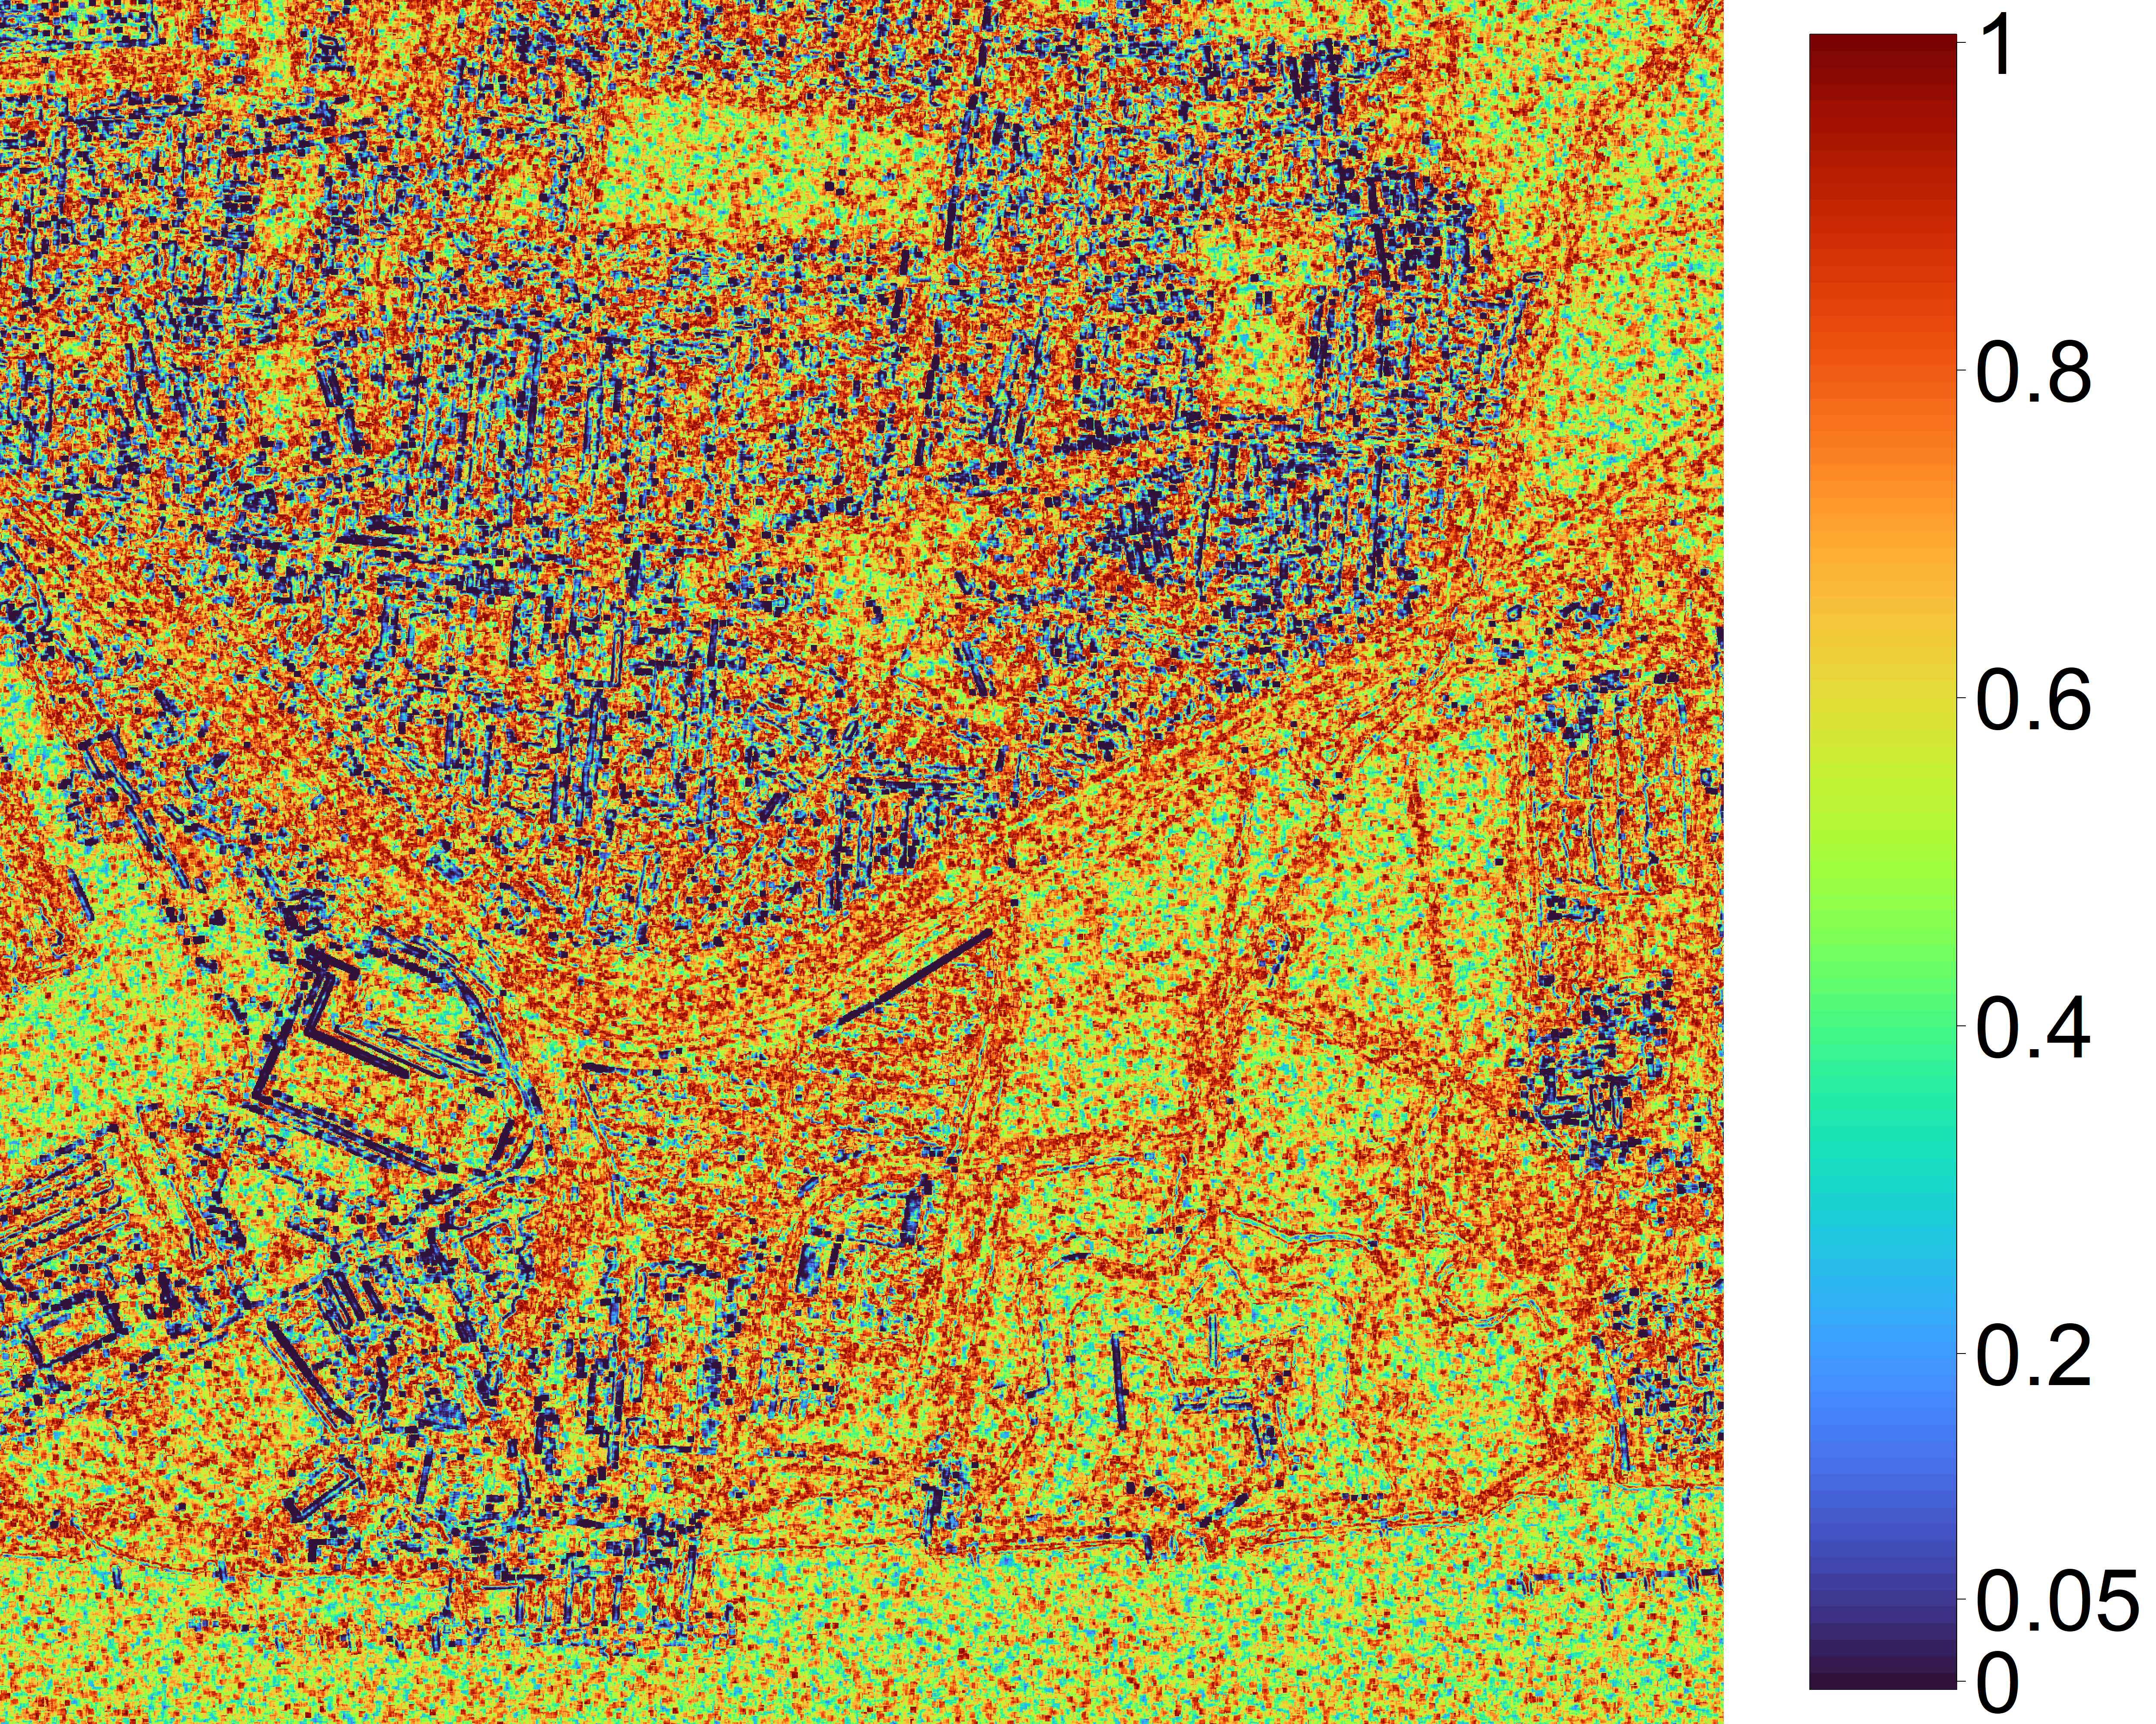
\includegraphics[width=\linewidth]{./Figures-R1/p-values_shannon-london_H1.png}
        \caption{$p$-value map for $\tiny{S_{\widetilde{H}_{\text{AO}}}}$ }
        \label{fig:london-shann}
    \end{subfigure}
    \hspace{0.00001\textwidth}
    \begin{subfigure}{0.145\textwidth}
        \includegraphics[width=\linewidth]{./Figures-R1/H_005_london_shannon.png}
        \caption{Binary map for $\small{S_{\widetilde{H}_{\text{AO}}}}$}
        \label{fig:london-005-shann}
    \end{subfigure}
    \caption{Detection of heterogeneous areas in a SAR image over London, UK: comparison with the tests $\small{S_{\widetilde{H}_{\lambda}}}$ and $\small{S_{\widetilde{H}_{\text{AO}}}}$.}
    \label{fig:london}
\end{figure*}

\begin{figure*}[hbt]
    \centering
        \begin{subfigure}{0.145\textwidth}
        \includegraphics[width=\linewidth]{./Figures-R1/munich_roi.png}
        \caption{SAR image}
        \label{fig:munich-sar}
    \end{subfigure}
    \hspace{0.00001\textwidth}
  \begin{subfigure}{0.137\textwidth}
        \includegraphics[width=\linewidth]{./Figures-R1/munich_optical.png}
        \caption{Optical image}
        \label{fig:munich-optical}
    \end{subfigure}
    \hspace{0.00001\textwidth}
    \begin{subfigure}{0.178\textwidth}
        \includegraphics[width=\linewidth]{./Figures-R1/p-values_renyi-munich_H.png}
        \caption{$p$-value map for $\small{S_{\widetilde{H}_{\lambda}}}$}
        \label{fig:munich-renyi}
    \end{subfigure}
    \hspace{0.00001\textwidth}
    \begin{subfigure}{0.144\textwidth}
        \includegraphics[width=\linewidth]{./Figures-R1/H_005_renyi_munich.png}
        \caption{Binary map for $\small{S_{\widetilde{H}_{\lambda}}}$}
        \label{fig:munich-005-renyi}
    \end{subfigure}
    \hspace{0.00001\textwidth}
    \begin{subfigure}{0.178\textwidth}
        \includegraphics[width=\linewidth]{./Figures-R1/p-values_shannon-munich_H.png}
        \caption{$p$-value map for $S_{\widetilde{H}_{\text{AO}}}$}
        \label{fig:munich-shann}
    \end{subfigure}
   \hspace{0.00001\textwidth}
    \begin{subfigure}{0.144\textwidth}
        \includegraphics[width=\linewidth]{./Figures-R1/H_005_shannon_munich.png}
        \caption{Binary map for $\small{S_{\widetilde{H}_{\text{AO}}}}$}
        \label{fig:munich-005-shann}
    \end{subfigure}
    \caption{Detection of heterogeneous areas in a SAR image over Munich, Germany: comparison with the tests $\small{S_{\widetilde{H}_{\lambda}}}$ and $\small{S_{\widetilde{H}_{\text{AO}}}}$.}
    \label{fig:munich}
\end{figure*}

\begin{figure*}[hbt]
    \centering
        \begin{subfigure}{0.145\textwidth}
        \includegraphics[width=\linewidth]{./Figures-R1/dublin_roi3.png}
        \caption{SAR image}
        \label{fig:dublin-sar}
    \end{subfigure}
    \hspace{0.00001\textwidth}
\begin{subfigure}{0.145\textwidth}
        \includegraphics[width=\linewidth]{./Figures-R1/dublin.png}
        \caption{Optical image}
        \label{fig:dublin-optical}
    \end{subfigure}
    \hspace{0.00001\textwidth}
    \begin{subfigure}{0.178\textwidth}
        \includegraphics[width=\linewidth]{./Figures-R1/p-values_renyi-dublin-H1.png}
        \caption{$p$-value map $\small{S_{\widetilde{H}_{\lambda}}}$}
        \label{fig:dublin-renyi}
    \end{subfigure}
    \hspace{0.00001\textwidth}
    \begin{subfigure}{0.144\textwidth}
        \includegraphics[width=\linewidth]{./Figures-R1/H_005_dublin_renyi.png}
        \caption{Binary map $\small{S_{\widetilde{H}_{\lambda}}}$}
        \label{fig:dublin-005-renyi}
    \end{subfigure}
    \hspace{0.00001\textwidth}
    \begin{subfigure}{0.178\textwidth}
        \includegraphics[width=\linewidth]{./Figures-R1/p-values_shannon-dublin-H1.png}
        \caption{$p$-value $\small{S_{\widetilde{H}_{\text{AO}}}}$}
        \label{fig:dublin-shann}
    \end{subfigure}
    \hspace{0.0000001\textwidth}
    \begin{subfigure}{0.144\textwidth}
        \includegraphics[width=\linewidth]{./Figures-R1/H_005_dublin-shannon.png}
        \caption{Binary $\small{S_{\widetilde{H}_{\text{AO}}}}$}
        \label{fig:dublin-005-shann}
    \end{subfigure}
    \caption{Detection of heterogeneous areas in a SAR image over Dublin Port, Ireland: comparison with the tests $\small{S_{\widetilde{H}_{\lambda}}}$ and $\small{S_{\widetilde{H}_{\text{AO}}}}$.}
    \label{fig:dublin}
\end{figure*}

\subsection{Quantitative Evaluation}\label{quantitative-evaluation}

\textcolor{blue}{Eight polygonal regions of interest (ROIs) were manually selected for
each scene (Figs.~\ref{fig:london-sar}-\ref{fig:dublin-sar}):
heterogeneous areas (red, class 1) and homogeneous areas (blue, class
0). These ROIs were rasterized to match the SAR resolution, forming a
partial ground truth. We thresholded the \(p\)-value maps at 0.05,
labeling each pixel as heterogeneous (1) or homogeneous (0) and then
compared these decision maps with the ground truth to compute: F1-score
(\(F_1\)), Kappa coefficient (\(\kappa\)), and overall accuracy (OA).
Table~\ref{tab:table_metrics} summarizes the results. Across all scenes,
the Rényi-based test outperformed Shannon's in all metrics, with notable
gains in London (\(F_1\): 0.695 vs.~0.617; \(\kappa\): 0.626 vs.~0.542),
highlighting its ability to capture heterogeneity under strong speckle
(single-look).}

\renewcommand{\arraystretch}{1.1}

\begin{table}[hbt]
\centering\centering
\caption{\label{tab:table_metrics}Quantitative measures of heterogeneity detection}
\resizebox{\ifdim\width>\linewidth\linewidth\else\width\fi}{!}{
\fontsize{7}{9}\selectfont
\begin{tabu} to \linewidth {>{\centering}X>{\centering}X>{\centering}X>{\centering}X>{\centering}X}
\toprule
\multicolumn{1}{c}{\textbf{Scene}} & \multicolumn{1}{c}{\textbf{Test}} & \multicolumn{1}{c}{$\bm{F_1}$} & \multicolumn{1}{c}{$\kappa$} & \multicolumn{1}{c}{\textbf{OA}}\\
\midrule
 & $S_{\widetilde{H}_{\lambda}}$ & \bm{$0.695$} & \bm{$0.626$} & \bm{$0.877$}\\

\multirow[b]{-2}{*}[\normalbaselineskip]{\centering\arraybackslash London} & $S_{\widetilde{H}_{\text{AO}}}$ & $0.617$ & $0.542$ & $0.854$\\
\cmidrule{1-5}
 & $S_{\widetilde{H}_{\lambda}}$ & \bm{$0.924$} & \bm{$0.861$} & \bm{$0.931$}\\

\multirow[b]{-2}{*}[\normalbaselineskip]{\centering\arraybackslash Munich} & $S_{\widetilde{H}_{\text{AO}}}$ & $0.883$ & $0.794$ & $0.897$\\
\cmidrule{1-5}
 & $S_{\widetilde{H}_{\lambda}}$ & \bm{$0.865$} & \bm{$0.753$} & \bm{$0.875$}\\

\multirow[b]{-2}{*}[\normalbaselineskip]{\centering\arraybackslash Dublin} & $S_{\widetilde{H}_{\text{AO}}}$ & $0.645$ & $0.464$ & $0.858$\\
\bottomrule
\end{tabu}}
\end{table}

\textcolor{blue}{Using the same ROIs as ground truth, we evaluated the continuous
\(p\)-value maps by computing receiver operating characteristic (ROC)
curves over all decision thresholds~(Fig.~\ref{fig:roc}). Each curve
plots the probability of detection (Pd) versus the probability of false
alarm (PFA). Pd reflects the proportion of heterogeneous pixels
correctly detected, while PFA represents the proportion of homogeneous
pixels misclassified as heterogeneous.}

\begin{figure}[hbt]
  \centering
  \includegraphics[width=0.49\textwidth]{Figures-R1/ROC1-1.pdf}
  \caption{ROC curves comparing the tests $S_{\widetilde{H}_{\lambda}}$ and $S_{\widetilde{H}_{\text{AO}}}$.}
  \label{fig:roc}
\end{figure}

\textcolor{blue}{The area under each ROC curve (AUC) quantifies global detection
performance. The Rényi-based test achieved higher AUCs across all
scenes---London: 0.963 vs.~0.776; Munich: 0.996 vs.~0.989; Dublin: 0.980
vs.~0.971---demonstrating superior robustness compared to the
Shannon-based test under various terrain conditions and textures.}

\section{Conclusions}\label{sec:conclusion}

This study presented a statistical approach based on Rényi entropy for
detecting heterogeneity in SAR images, distinguishing between fully
developed speckle and heterogeneous clutter. The proposed test was
validated with synthetic experiments via a Monte Carlo study,
demonstrating that it effectively controls the probability of Type~I
error while maintaining high detection performance that improves with
sample size.

\textcolor{blue}{Using SAR data, we compared the Rényi-based test with a Shannon-based counterpart through $p$-value maps and binary decisions. Visual analysis showed greater sensitivity of the Rényi-based test to textural variations.
Quantitative evaluation with ground truth ROIs and standard classification metrics confirmed the superior performance of the Rényi-based test across all scenes.}

\textcolor{blue}{Although machine learning-based SAR classifiers are widely used, our focus is on interpretable, statistically grounded methods that yield analytical significance measures. This makes them suitable for rapid detection, screening, and environments with limited data availability.}

\textcolor{blue}{Future work will explore the integration of the improved Rényi estimator into SAR classification pipelines, both supervised and unsupervised, extending its utility beyond heterogeneity testing.}

\section*{References}\label{references}
\addcontentsline{toc}{section}{References}

\phantomsection\label{refs}
\begin{CSLReferences}{0}{0}
\bibitem[\citeproctext]{ref-Mondini2021}
\CSLLeftMargin{{[}1{]} }%
\CSLRightInline{A. C. Mondini, F. Guzzetti, K.-T. Chang, O. Monserrat,
T. R. Martha, and A. Manconi,
{``\href{https://doi.org/10.1016/j.earscirev.2021.103574}{Landslide
failures detection and mapping using synthetic aperture radar: Past,
present and future},''} \emph{Earth-Science Reviews}, vol. 216, p.
103574, 2021. }

\bibitem[\citeproctext]{ref-Zeng2020}
\CSLLeftMargin{{[}2{]} }%
\CSLRightInline{Z. Zeng \emph{et al.},
{``\href{https://doi.org/10.1016/j.jhydrol.2019.124377}{Towards high
resolution flood monitoring: An integrated methodology using passive
microwave brightness temperatures and sentinel synthetic aperture radar
imagery},''} \emph{Journal of Hydrology}, vol. 582, p. 124377, 2020. }

\bibitem[\citeproctext]{ref-Baraha2023}
\CSLLeftMargin{{[}3{]} }%
\CSLRightInline{S. Baraha and A. K. Sahoo,
{``\href{https://doi.org/10.1016/j.sigpro.2023.109156}{Synthetic
aperture radar image and its despeckling using variational methods: A
review of recent trends},''} \emph{Signal Processing}, vol. 212, p.
109156, 2023. }

\bibitem[\citeproctext]{ref-Nascimento2014}
\CSLLeftMargin{{[}4{]} }%
\CSLRightInline{A. D. C. Nascimento, M. M. Horta, A. C. Frery, and R. J.
Cintra, {``Comparing edge detection methods based on stochastic
entropies and distances for {PolSAR} imagery,''} \emph{{IEEE} Journal of
Selected Topics in Applied Earth Observations and Remote Sensing}, vol.
7, no. 2, pp. 648--663, 2014. }

\bibitem[\citeproctext]{ref-Nobre2016}
\CSLLeftMargin{{[}5{]} }%
\CSLRightInline{R. H. Nobre, F. A. A. Rodrigues, R. C. P. Marques, J. S.
Nobre, J. F. S. R. Neto, and F. N. S. Medeiros,
{``\href{https://doi.org/10.1109/lsp.2016.2606760}{SAR image
segmentation with {R}ényi's entropy},''} \emph{IEEE Signal Processing
Letters}, vol. 23, no. 11, pp. 1551--1555, 2016. }

\bibitem[\citeproctext]{ref-Chan2022}
\CSLLeftMargin{{[}6{]} }%
\CSLRightInline{D. Chan, J. Gambini, and A. C. Frery,
{``\href{https://doi.org/10.3390/rs14030509}{Entropy-based non-local
means filter for single-look SAR speckle reduction},''} \emph{Remote
Sensing}, vol. 14, no. 3, p. 509, 2022. }

\bibitem[\citeproctext]{ref-Shannon1948}
\CSLLeftMargin{{[}7{]} }%
\CSLRightInline{C. E. Shannon, {``A mathematical theory of
communication,''} \emph{The Bell System Technical Journal}, vol. 27, no.
3, pp. 379--423, 1948. }

\bibitem[\citeproctext]{ref-Cassetti2022}
\CSLLeftMargin{{[}8{]} }%
\CSLRightInline{J. Cassetti, D. Delgadino, A. Rey, and A. C. Frery,
{``Entropy estimators in {SAR} image classification,''} \emph{Entropy},
vol. 24, no. 4, p. 509, 2022. }

\bibitem[\citeproctext]{ref-Gallet2024}
\CSLLeftMargin{{[}9{]} }%
\CSLRightInline{M. Gallet, A. Mian, and A. Atto,
{``\href{https://doi.org/10.1109/icassp48485.2024.10448227}{Renyi
divergences learning for explainable classification of {SAR} image
pairs},''} in \emph{2024 {IEEE} {I}nternational {C}onference on
{A}coustics, {S}peech and {S}ignal {P}rocessing {(ICASSP)}}, 2024, pp.
7445--7449. }

\bibitem[\citeproctext]{ref-Parikh2019}
\CSLLeftMargin{{[}10{]} }%
\CSLRightInline{H. Parikh, S. Patel, and V. Patel,
{``\href{https://doi.org/10.1080/19479832.2019.1655489}{Classification
of {SAR} and {PolSAR} images using deep learning: A review},''}
\emph{International Journal of Image and Data Fusion}, vol. 11, no. 1,
pp. 1--32, 2019. }

\bibitem[\citeproctext]{ref-Frery2024}
\CSLLeftMargin{{[}11{]} }%
\CSLRightInline{A. C. Frery, J. Alpala, and A. D. C. Nascimento,
{``\href{https://doi.org/10.3390/rs16111973}{Identifying heterogeneity
in {SAR} data with new test statistics},''} \emph{Remote Sensing}, vol.
16, no. 11, p. 1973, 2024. }

\bibitem[\citeproctext]{ref-Frery1997}
\CSLLeftMargin{{[}12{]} }%
\CSLRightInline{A. C. Frery, H.-J. Muller, C. C. F. Yanasse, and S. J.
S. SantAnna, {``A model for extremely heterogeneous clutter,''}
\emph{{IEEE} Transactions on Geoscience and Remote Sensing}, vol. 35,
no. 3, pp. 648--659, 1997. }

\bibitem[\citeproctext]{ref-AlLabadi2024}
\CSLLeftMargin{{[}13{]} }%
\CSLRightInline{L. Al-Labadi, Z. Chu, and Y. Xu,
{``\href{https://doi.org/10.1007/s00180-024-01507-z}{Advancements in
{R}ényi entropy and divergence estimation for model assessment},''}
\emph{Computational Statistics}, 2024. }

\bibitem[\citeproctext]{ref-Alpala2024}
\CSLLeftMargin{{[}14{]} }%
\CSLRightInline{R. J. Alpala, A. D. C. Nascimento, and A. C. Frery,
{``\href{https://doi.org/10.1109/migars61408.2024.10544448}{Identifying
departures from the fully developed speckle hypothesis in intensity
{SAR} data with non-parametric estimation of the entropy},''} in
\emph{2024 {I}nternational {C}onference on {M}achine {I}ntelligence for
{G}eo{A}nalytics and {R}emote {S}ensing ({MIGARS})}, 2024, pp. 1--4. }

\bibitem[\citeproctext]{ref-vasicek1976test}
\CSLLeftMargin{{[}15{]} }%
\CSLRightInline{O. Vasicek, {``A test for normality based on sample
entropy,''} \emph{Journal of the Royal Statistical Society Series B:
Statistical Methodology}, vol. 38, no. 1, pp. 54--59, 1976. }

\bibitem[\citeproctext]{ref-IbrahimAlOmari2014}
\CSLLeftMargin{{[}16{]} }%
\CSLRightInline{A. I. Al-Omari, {``Estimation of entropy using random
sampling,''} \emph{Journal of Computational and Applied Mathematics},
vol. 261, pp. 95--102, 2014. }

\end{CSLReferences}


% Can use something like this to put references on a page
% by themselves when using endfloat and the captionsoff option.
\ifCLASSOPTIONcaptionsoff
  \newpage
\fi

% trigger a \newpage just before the given reference
% number - used to balance the columns on the last page
% adjust value as needed - may need to be readjusted if
% the document is modified later
%\IEEEtriggeratref{8}
% The "triggered" command can be changed if desired:
%\IEEEtriggercmd{\enlargethispage{-5in}}

% Uncomment when use biblatex with style=ieee
%\renewcommand{\bibfont}{\footnotesize} % for IEEE bibfont size

\pagebreak[3]
% that's all folks
\end{document}

